% WWW 2027 Demonstrations. Compile with: tectonic main.tex
\documentclass[sigconf,screen,review]{acmart}
\usepackage{amsmath}
\usepackage{booktabs}
\usepackage{tabularx}
\usepackage{balance}
\usepackage{tikz}
\usetikzlibrary{arrows.meta,positioning,calc}
\setcopyright{none}
\settopmatter{printacmref=false}
\acmDOI{}
\acmISBN{}
\acmConference[WWW '27]{The ACM Web Conference 2027}{May 10--14, 2027}{Dublin, Ireland}
\acmYear{2027}
\copyrightyear{2027}
\newcommand{\sys}{DeepShovel~2.0}
\definecolor{navy}{HTML}{17324D}
\definecolor{teal}{HTML}{087F8C}
\definecolor{amber}{HTML}{AA6425}
\definecolor{pale}{HTML}{EDF6F6}
\emergencystretch=1em
\begin{document}
\title[DeepShovel 2.0: Scientific Reasoning Networks]{\sys: A Scientific Reasoning Network for Evidence-Grounded Verification and Discovery}
\author{Haoxiang Zhang}
\email{1227538797@sjtu.edu.cn}
\orcid{0009-0006-4255-0811}
\affiliation{\institution{Shanghai Jiao Tong University}\city{Shanghai}\country{China}}
\author{Jiaxin Ding}
\authornote{Corresponding author.}
\email{jiaxinding@sjtu.edu.cn}
\orcid{0000-0002-0009-9237}
\affiliation{\institution{Shanghai Jiao Tong University}\city{Shanghai}\country{China}}
\renewcommand{\shortauthors}{Zhang and Ding}

\begin{abstract}
Scientific knowledge is reusable when a conclusion remains connected to the evidence, assumptions, and inferential steps that justify it. We present \sys{}, an operational system that reconstructs the principal arguments of scientific papers and integrates them into a curated domain reasoning network. Each argument retains its jointly required premises, applicability conditions, and traceable links to source passages, data, tables, and figures. Reasoning-aware retrieval and retrieval-augmented generation assemble supporting arguments and applicable counterevidence, enabling verification of individual claims and the interdependent conclusions of one or more papers. Research agents operate on the same network to derive candidate claims, challenge their premises, and refine research strategies through successive investigations. A Codex-orchestrated geoscience study screened 48 candidates across eight rounds and produced a reproducible manuscript on regional transfer of a seawater rare-earth-element pH calibration. The demonstration connects paper understanding, premise-level verification, and agent-driven exploration through a common, inspectable scientific argument model.
\end{abstract}
\ccsdesc[500]{Information systems~Digital libraries and archives}
\ccsdesc[500]{Computing methodologies~Knowledge representation and reasoning}
\ccsdesc[300]{Information systems~Retrieval models and ranking}
\keywords{scientific reasoning networks, argument reconstruction, evidence provenance, claim verification, retrieval-augmented generation, research agents}
\maketitle

\section{Introduction}
Scientific conclusions depend on observations, assumptions, and inferential steps. Reuse requires recovering why they hold and where they apply: a calibration's original fit, for example, does not establish its transferability. 

\sys{} makes the \emph{source-grounded scientific argument} the reusable unit of knowledge. It reconstructs each admitted paper's research question, main claims, and inferential dependencies, then connects these arguments across selected domain literature. The network preserves the conditions under which conclusions support, qualify, or challenge one another. It supports two complementary operations: tracing a conclusion backward to its justification, and extending grounded premises forward into new, testable inferences.

For the scholarly Web, publications, figures, tables, and data become addressable components of cross-document reasoning. Source links connect an answer to an inference and its original evidence. The running system is at \url{https://deepshovel.iiot-shxt.xyz}. Code, fixed cases, an English walkthrough, and the research reproduction package are released at \url{https://github.com/spiderLL2002/deepshovel}, tag \texttt{www2027-artifact-v1.1.0}. A service snapshot on 27 October 2026 reported 9,506 active paper families and 41,092 active claims. Expert review of development questions and datasets and additional spot checks support quality control; these activity counts do not imply individually expert-certified inferences.

\paragraph{Contribution and positioning.}
GeoDeepShovel supports scientific database construction~\cite{geodeepshovel}; SciFact formalizes claim verification with evidence rationales~\cite{scifact}. Argument Web benchmarks prediction of argumentative relations across discourse units~\cite{argumentweb}; GraphRAG supports graph-based synthesis~\cite{graphrag}. ResearchAgent iteratively develops research ideas~\cite{researchagent}; DeepEvidence coordinates breadth/depth exploration across biomedical knowledge sources and records an evolving evidence graph~\cite{deepevidence}. Our contribution is \emph{continuity of scientific justification}: the joint inputs and applicability conditions of a paper's internal inferences survive retrieval, while research records connect new deductions to sources and analyses. The demonstration exposes the difference between a short source path and preserved joint dependencies, and follows retrieved arguments into research decisions. 

\begin{figure*}[t]
\centering
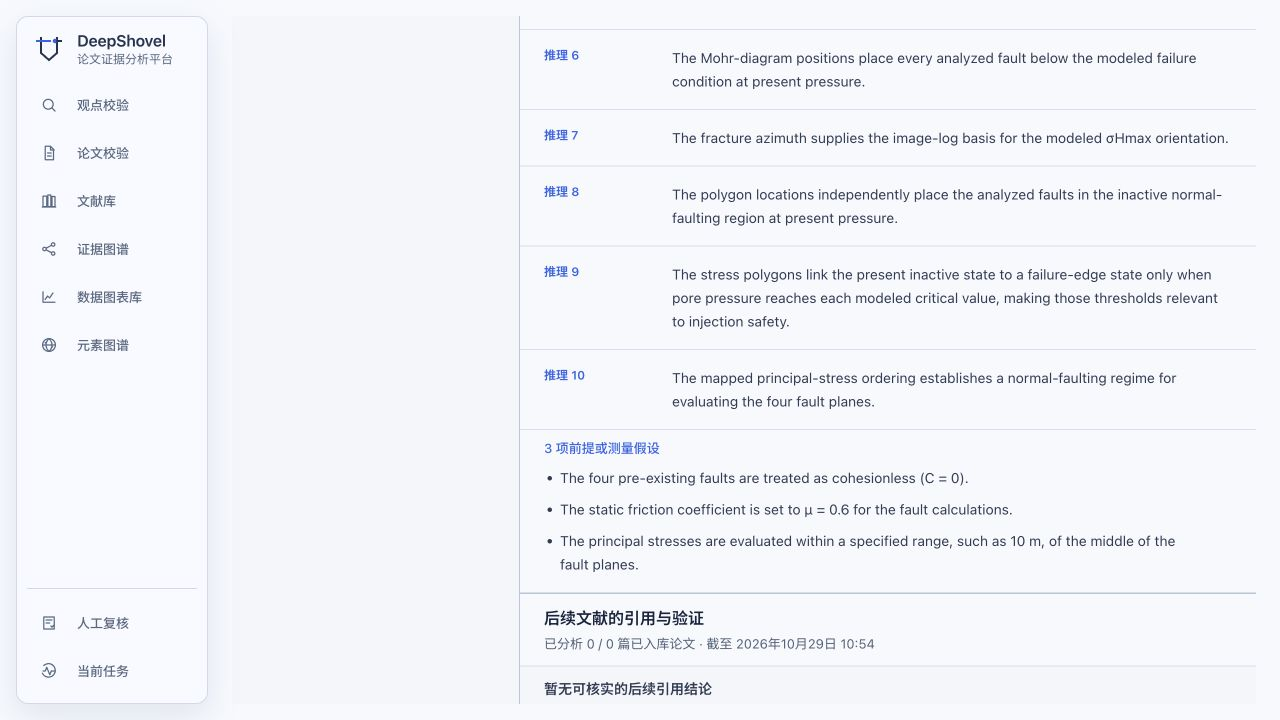
\includegraphics[width=0.93\textwidth,trim={520bp 125bp 25bp 430bp},clip]{../artifact/live-demo/04-assumptions.jpg}
\caption{Actual F2 inspector with its three expanded assumptions. The release provides uncropped screenshots, the exact query, original-page inspection, and an English walkthrough.}
\Description{The production interface shows three assumptions: zero cohesion, friction 0.6, and stress sampling near the middle of the fault plane.}
\label{fig:architecture}
\end{figure*}

\section{Compiling a Domain Reasoning Network}
\label{sec:network}
Figure~\ref{fig:architecture} shows conditions retained in the running claim inspector.
\paragraph{Recover the paper's scientific meaning.}
Ingestion parses sections, equations, references, tables, figure panels, captions, and supplementary data into addressable source objects. Reconstruction follows the paper's main reasoning routes: question $\rightarrow$ methods and assumptions $\rightarrow$ observations $\rightarrow$ intermediate interpretations $\rightarrow$ conclusions. Backward reconstruction gathers claim premises; forward reconstruction checks how observations support intermediate and final claims.

A reasoning step is represented as
\begin{equation}
r=(P_r,A_r,w_r,c_r,\sigma_r,\pi_r),
\end{equation}
where $P_r$ contains jointly required premises, $A_r$ assumptions, $w_r$ the inferential warrant or analysis, $c_r$ the conclusion, $\sigma_r$ applicability conditions, and $\pi_r$ provenance. An explicit inference node joins all co-premises. Arguments may branch through multiple observations or converge through intermediate results; one path to a conclusion can omit other required inputs.

In the stored Asmari graph~\cite{asmari}, \texttt{reason.f2.evidence} receives two \texttt{premise\_for} and three \texttt{assumption\_for} inputs (Figure~\ref{fig:architecture}). Its downstream pressure inference also requires current-stress and critical-pressure reasoning. This explicit dependency set explains why retrieving one source path is insufficient.

Scope records material or population, setting, method, comparison, and spatial or temporal range. Reconstruction preserves quantifiers and negation and distinguishes an observation, an association, a mechanistic interpretation, and a prediction. Moving between these levels is itself an inference requiring justification. Provenance binds evidence to a document version and a passage, equation, table cell, figure panel, or dataset record. Numerical observations retain units and uncertainty; figure interpretations retain axes, captions, and experimental context. Author-stated arguments, reconstructed links, and agent-proposed inferences have distinct origins. Missing premises remain visible obligations.



\paragraph{Compose arguments with their conditions intact.}
Cross-paper alignment compares proposition meaning and scope, retaining individual claim instances and support, challenge, qualification, and dependency relations. Combining findings introduces a bridge inference with inspectable compatibility assumptions. Contradictions may target an observation, an assumption, or the warrant connecting premises to a conclusion.

Evidence lineage groups paper versions, reused datasets, and derivative analyses to distinguish repeated measurements from independent confirmation. Source fidelity, premise coverage, methodological adequacy, scope, and counterevidence inform review. Displayed confidence is a model assessment, not a calibrated truth probability.

\paragraph{Execution boundary.}
Language-model reconstruction assigns \texttt{premise\_for} and \texttt{assumption\_for} inputs to explicit inference nodes; these assignments distinguish required inputs from background. Separate inference nodes preserve alternative routes. Deterministic graph operations follow the recorded assignments and source identities. A warrant is a readable justification or analysis reference, not a machine-checked proof. Scope judgments combine model interpretation with guards: proposed contradictions with disjoint or unknown scope are downgraded to related evidence. Different free-text scientific labels alone yield unknown scope. Source review and appropriate analyses establish scientific adequacy.

\section{Reasoning-Level Retrieval and Verification}
\label{sec:verification}
\paragraph{Retrieve the justification of an answer.}
Requests identify a target proposition, scope, and evidential needs. Lexical/semantic retrieval recalls claims and observations; reranking prioritizes relevance and applicability. Support and counterevidence searches cover incompatible observations, alternative mechanisms, failed transfers, and challenged assumptions.

The search list offers a short preview. Opening a claim executes backward dependency expansion, following all represented premise and assumption inputs and their grounding links. The detail response retains the resulting \emph{argument bundle} and marks \texttt{truncated} if its depth bound (default 32) stops expansion. This checks completeness relative to recorded dependencies; it cannot detect scientific premises never extracted from the source. Synthesis budgets and scientific sufficiency are separate from this explicit traversal bound.

RAG synthesizes a scoped answer with assertions linked to reasoning steps and evidence. Retrieval prioritizes premises needed to justify a proposition or change its interpretation.

\paragraph{Locate the disagreement inside the argument.}
Verification distinguishes support, contradiction, qualification, and unresolved evidence. A counterexample must address the claimed scope; another regime may instead challenge a generalization. The challenged observation, assumption, or inference locates the disagreement. Dependency traversal connects a paper's principal claims; alignment across papers exposes differences in data, methods, or applicability. Alternative support can preserve a conclusion when one route fails.

\paragraph{Executable checks of recorded premises.}
The release executes the unchanged production detail expander on all seven claims in the saved Asmari graph~\cite{asmari}. An independent fixed-point traversal supplies the reference edge sets: all seven full expansions match. For F2, the search preview retains 1/18 recorded premise edges and 1/3 assumption edges; the detail expansion retains \textbf{18/18 and 3/3}, in 41 entities and 37 edges. Thus users can recover the three-method agreement, current-stress reasoning, and three assumptions omitted by a short trace. This directly checks joint-input preservation, beyond path existence.

Depth limits 1, 2, and 3 produce 21 bounded runs, all marked truncated; all 19 runs omitting premise or assumption edges are flagged. Three controlled missing-input mutations are rejected by the production validator. A retained negative example also shows that an unrecorded internal dependency can pass structural validation. These are checks on one paper, not extraction-accuracy estimates. The earlier 20-result structural cohort and 33-node auxiliary export remain separately labeled in the release.

The live walkthrough opens F2's original page 11, reasoning steps, and assumptions (Figure~\ref{fig:architecture}). Source inspection qualifies the imported scalar 55 as the approximate 55--57\,MPa maximum sustainable pore pressure under zero cohesion and friction 0.6, rather than a pressure increment or statistical interval. A known wrong-column rectangle remains documented; page and quotation inspection are required. The release also preserves three Nd queries where the same candidate changes from related to supporting to related as the target changes. These are inspectable model decisions; synthetic scope-guard fixtures are labeled separately.

\begin{figure*}[t]
\centering
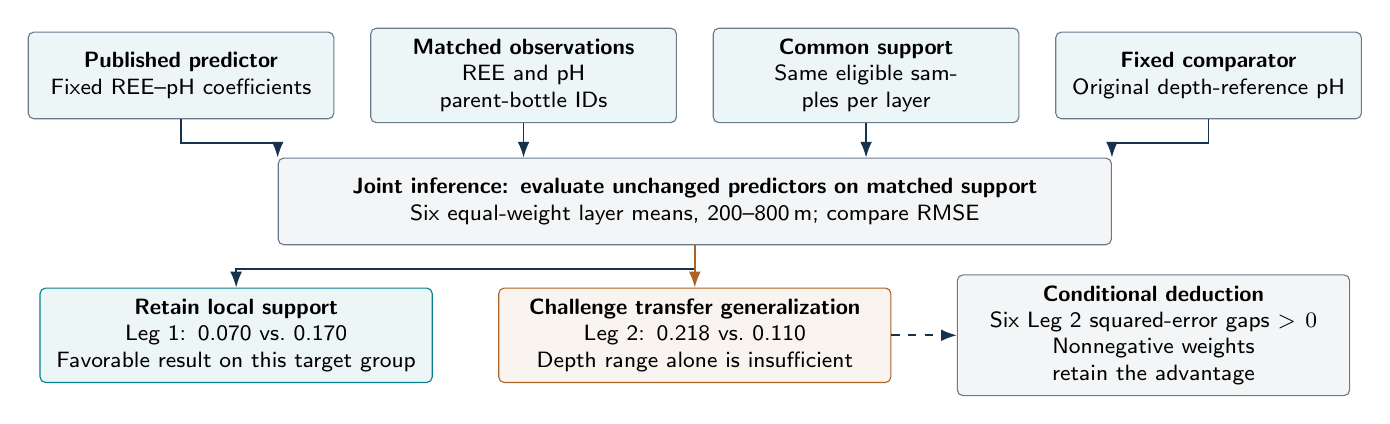
\begin{tikzpicture}[font=\sffamily\footnotesize,>=Latex,
nodebox/.style={draw=navy!65,rounded corners=2pt,align=center,inner sep=4pt,minimum height=11mm},
arr/.style={->,draw=navy,semithick}]
\node[nodebox,fill=pale,text width=36mm] (m) at (0,0) {\textbf{Published predictor}\\Fixed REE--pH coefficients};
\node[nodebox,fill=pale,text width=36mm] (d) at (4.35,0) {\textbf{Matched observations}\\REE and pH parent-bottle IDs};
\node[nodebox,fill=pale,text width=36mm] (s) at (8.7,0) {\textbf{Common support}\\Same eligible samples per layer};
\node[nodebox,fill=pale,text width=36mm] (b) at (13.05,0) {\textbf{Fixed comparator}\\Original depth-reference pH};
\node[nodebox,fill=navy!5,text width=103mm] (r) at (6.525,-1.6) {\textbf{Joint inference: evaluate unchanged predictors on matched support}\\Six equal-weight layer means, 200--800\,m; compare RMSE};
\draw[arr] (m.south)--++(0,-3mm)-|(r.north west);
\draw[arr] (d.south)--(r.north -| d.south);
\draw[arr] (s.south)--(r.north -| s.south);
\draw[arr] (b.south)--++(0,-3mm)-|(r.north east);
\node[nodebox,draw=teal,fill=pale,text width=47mm] (a) at (0.7,-3.3) {\textbf{Retain local support}\\Leg 1: 0.070 vs.\ 0.170\\Favorable result on this target group};
\node[nodebox,draw=amber,fill=amber!7,text width=47mm] (c) at (6.525,-3.3) {\textbf{Challenge transfer generalization}\\Leg 2: 0.218 vs.\ 0.110\\Depth range alone is insufficient};
\node[nodebox,fill=navy!5,text width=47mm] (h) at (12.35,-3.3) {\textbf{Conditional deduction}\\Six Leg 2 squared-error gaps $>0$\\Nonnegative weights retain the advantage};
\draw[arr] (r.south)--++(0,-3mm)-|(a.north);
\draw[arr,draw=amber] (r.south)--(c.north);
\draw[arr,dashed] (c.east)--(h.west);
\end{tikzpicture}
\caption{Instantiated reasoning structure for the completed GP15 investigation. The four top-row premises jointly warrant the comparison. The adverse branch challenges a generalization posed for verification, while the source's original calibration and the favorable local result remain available. The final box holds for the same unperturbed layer means; changing within-layer support requires a new analysis.}
\Description{Four joint premises feed a fixed-model comparison: original coefficients, matched observations, common sampling support, and a fixed depth reference. A favorable branch retains local support, an adverse branch challenges transfer, and a dashed arrow marks a scoped deduction about arbitrary nonnegative depth weights.}
\label{fig:argument}
\end{figure*}

\section{Agents for Discovery and Recursive Improvement}
\label{sec:agents}
Agents retrieve a target's justification, identify an unresolved transition, propose a conditional inference, and seek counterexamples and prior work. Candidates retain their derivation, bridging assumptions, and discriminating analysis. Task-level recursive self-improvement (RSI) records feedback-driven revisions to the investigation procedure.

\paragraph{An executed geoscience investigation.}
A Codex-orchestrated run screened 48 candidates over eight rounds in rare-earth geochemistry and ocean anoxic-event research, advancing one to a reproducible manuscript. In a documented screening decision, DeepShovel returned Hongo et al.'s~\cite{hongo} scoped REE--Mg mixing argument. The agent followed its source chain to the original methods and Figures 10--12, established prior overlap, and retained the filtered/unfiltered sampling distinction. The candidate record explicitly cites this source as strengthening the rejection of REE-R7-02. Released request timestamps, returned argument identifiers, PDF hash, and decision excerpts expose that contribution to research selection. The surviving question tested regional transfer of a published seawater REE--pH calibration~\cite{lin2024}.

The run combined DeepShovel retrieval and claim comparison with original publications and public GEOTRACES GP15 observations~\cite{gp15}. REE and pH were matched by parent-bottle identity, with distinct filtered/unfiltered analytical aliquots. The target, calibration, and depth reference use total-scale pH at 25$^\circ$C and surface pressure; no basis conversion was needed. The published chemical predictor and its original depth reference were fixed before comparison. Across six 100-m layers between 200 and 800\,m, their error ordering reversed between the two station groups (Table~\ref{tab:case}). This produced a precise claim: retaining the original depth interval did not ensure improvement over the original reference on the sampled support. Figure~\ref{fig:argument} makes the joint premises and the challenged generalization explicit.



\begin{table}[t]
\caption{Recorded research outcome: RMSE in pH units across six equal-weight layer means. Both methods use the same eligible samples within each layer. These errors describe the geochemical comparison.}
\label{tab:case}
\centering
\begin{tabular}{@{}lrrr@{}}
\toprule
GP15 group & Bottles / stations & REE model & Depth reference\\
\midrule
Leg 1 & 24 / 6 & 0.070 & 0.170\\
Leg 2 & 55 / 8 & 0.218 & 0.110\\
\bottomrule
\end{tabular}
\end{table}

The research record also contains a deductive extension. The Leg~2 layerwise squared-error differences $d_i=e_{\mathrm{REE},i}^2-e_{\mathrm{ref},i}^2$, in ascending depth order, are 0.07285, 0.05368, 0.05320, 0.02076, 0.00694, and 0.00545\,pH$^2$ (rounded). Hence $\sum_i w_i d_i>0$ for any $w_i\geq0$, $\sum_iw_i=1$: reweighting these same layer means cannot reverse the reference's advantage. The final claim--source map stores this as C12, binds it to the hashed layer-difference table, and restricts it to unchanged within-layer support. C03 separately binds the empirical RMSEs to their aggregate and layer records. Codex persists this claim ledger and its source maps in the research workspace. The propositions, with their scope, are sent as text to DeepShovel for itemwise comparison; its returned assessments are stored alongside the local analysis. A released lineage index joins the source-graph PDF hash to the research source-input file, frozen protocol, and C01/C03/C12 file hashes. This index was assembled from existing records for publication; graph and research-ledger identifiers remain separate, and automatic reinsertion is not asserted. 

The run also records an actual procedure revision. A Codex-coordinated review proposed stricter uncertainty reporting to require at least six station labels and 90\% complete-support resamples, and to suppress aggregate comparisons when a station deletion removed an originally represented layer. Codex incorporated these rules into the frozen analysis protocol; the subsequent deterministic run applied them. This is inspectable task-level RSI: feedback changes a reusable analysis procedure before its results are generated.

The public package includes exact model coefficients, depth-reference values, sample joins, the frozen protocol, manuscript, and claim maps. A fresh ten-stage run regenerated 76 reference files byte-identically. Sensitivities preserve the error ordering under four aggregation choices, station deletion, and alternate treatment of one unresolved depth. DeepShovel's seven final claim comparisons reported incomplete literature coverage and accepted no comparable literature relation. Codex-led source inspection established model definitions and sample identity; deterministic analysis supplied numerical support for the local claim. These distinct evidence channels remain labeled. The episode demonstrates completed research and procedure refinement; it does not isolate a performance gain from RSI.

\section{Interactive Demonstration}
\label{sec:demo}
Attendees trace a published argument to a tested claim, controlling the comparison scope and next research question.

\paragraph{1. Inspect a paper's reasoning (live).}
Paste the released F2 query into the Web workbench. Open the representative paper, inspect the 55--57\,MPa claim, expand its observations, reasoning steps and three assumptions, and open original page 11. Compare the short search preview with the complete recorded dependency set. The English guide translates the current Chinese controls and links each action to a real screenshot.

\paragraph{2. Test scope and completeness (live and replay).}
Change the query's setting or request counterevidence in the live service. Inspect the retained scope and relation explanations. Then replay the fixed Nd query trio and execute the released Asmari expansion with a lower depth bound: the response explicitly reports truncation. Full dependencies, short previews, and controlled invalid inputs are separately available for inspection.

\paragraph{3. Follow evidence into research (saved and executable).}
Open the Hongo retrieval-to-decision trace, then follow the GP15 source hash into the frozen protocol and C03/C12 outputs. Recompute the numerical claims locally; inspect the procedure revision and resulting manuscript. Attendees can request new counterevidence or propose an independent station group through the connected agent. New scientific investigations are not represented as instant replay results.

\paragraph{Venue operation and reproducibility.}
A laptop and browser run the live service alongside the research workspace. New retrieval and agent calls require connectivity and configured services. The tagged repository supplies full application source, fixed graphs, licensed sources, interface captures, English instructions, checkers, and locked dependencies. Key-free checks replay dependencies and research calculations; model outputs remain labeled saved observations. Fixed materials remain usable offline after setup, including SHA-256-verified restoration of two supporting inputs from their providers.

\balance
\section{Ethical Use of Data}
Publications and research data are used subject to their licenses and access permissions. Attribution, source versions, and derived-data provenance are retained. Expert-reviewed questions and datasets and spot checks support quality control; generated hypotheses retain their provisional status. The example reanalyzes public geochemical measurements and includes no human-subject experiment. Assessments concern scientific claims and applicability, not researchers' integrity.

\begin{thebibliography}{10}
\bibitem{geodeepshovel}
Shao Zhang et al. 2023. GeoDeepShovel: A platform for building scientific database from geoscience literature with AI assistance. \emph{Geoscience Data Journal} 10, 4, 519--537. \url{https://doi.org/10.1002/gdj3.186}
\bibitem{scifact}
David Wadden et al. 2020. Fact or Fiction: Verifying Scientific Claims. In \emph{EMNLP}, 7534--7550. \url{https://doi.org/10.18653/v1/2020.emnlp-main.609}
\bibitem{argumentweb}
Florian Ruosch, Cristina Sarasua, and Abraham Bernstein. 2025. Mining Inter-Document Argument Structures in Scientific Papers for an Argument Web. \emph{Transactions on Graph Data and Knowledge} 3, 3, Article 4. \url{https://doi.org/10.4230/TGDK.3.3.4}
\bibitem{graphrag}
Darren Edge et al. 2024. From Local to Global: A Graph RAG Approach to Query-Focused Summarization. \emph{arXiv:2404.16130}. \url{https://arxiv.org/abs/2404.16130}
\bibitem{researchagent}
Jinheon Baek, Sujay Kumar Jauhar, Silviu Cucerzan, and Sung Ju Hwang. 2025. ResearchAgent: Iterative Research Idea Generation over Scientific Literature with Large Language Models. In \emph{NAACL}, 6709--6738. \url{https://doi.org/10.18653/v1/2025.naacl-long.342}
\bibitem{deepevidence}
Zifeng Wang et al. 2026. Empowering biomedical evidence exploration and synthesis with deep knowledge graph research. \emph{Nature Machine Intelligence} 8, 1142--1156. \url{https://doi.org/10.1038/s42256-026-01266-0}
\bibitem{lin2024}
Ping-Chun Lin and David C. Catling. 2024. The Rare Earth Element Distribution in Marine Carbonates as a Potential Proxy for Seawater pH on Early Earth. \emph{American Journal of Science} 324, Article 10. \url{https://doi.org/10.2475/001c.118215}
\bibitem{gp15}
BCO-DMO. GEOTRACES GP15 rare earth element and pH datasets. REE: \url{https://doi.org/10.26008/1912/bco-dmo.932161.1}, \url{https://doi.org/10.26008/1912/bco-dmo.932559.1}; pH: \url{https://doi.org/10.26008/1912/bco-dmo.838157.2}, \url{https://doi.org/10.26008/1912/bco-dmo.838173.2}.
\bibitem{asmari}
Majid Taghipour et al. 2019. Estimation of the current stress field and fault reactivation analysis in the Asmari reservoir, SW Iran. \emph{Petroleum Science} 16, 513--526. \url{https://doi.org/10.1007/s12182-019-0331-9}
\bibitem{hongo}
Yayoi Hongo et al. 2007. Rare Earth Elements in the hydrothermal system at Okinawa Trough back-arc basin. \emph{Geochemical Journal} 41, 1, 1--15. \url{https://doi.org/10.2343/geochemj.41.1}
\end{thebibliography}
\end{document}
